\documentclass{beamer}
\usepackage{graphicx}
\usepackage{tikz}
\usetikzlibrary{shapes,arrows}
\usepackage{tikz}
%\usecolortheme{seahorse}
  \setbeamertemplate{footline}[page number]
\usepackage{multirow}
\setbeamertemplate{navigation symbols}{}
\setbeamertemplate{frametitle}[default][center]
\setbeamerfont{frametitle}{shape=\scshape}
\usepackage{color}

\usepackage{csquotes}

\usepackage{xcolor}

\usepackage[flushleft]{threeparttable}

{\title{\textsc{Econ 352 - Credit Market Imperfections - Credit Frictions, Financial Crises, and Social Security} \\ \tiny (See Williamson Ch. 10)}
\author{Trevor S. Gallen}
\date{}
\begin{document}
\renewcommand*{\inserttotalframenumber}{\pageref{lastframe}}


\setbeamertemplate{caption}{\raggedright\insertcaption\par}

\begin{frame}
\titlepage
\end{frame}

\begin{frame}
\frametitle[alignment=center]{Introduction}
\begin{itemize}
\item Chapter 9 started thinking about credit markets--smoothing behavior
\bigskip
\item And one big prediction from Chapter 9 was the Ricardian Equivalence theorem!
\bigskip
\begin{itemize}
\item The timing of lump-sum taxes doesn't matter if it doesn't change NPV income
\end{itemize}
\bigskip
\item But we make a big assumption: perfect credit markets
\bigskip
\item In this chapter, we add frictions: asymmetric information, and limited committment
\bigskip
\item They'll help us better understand some modern events (2008, 2022(?))
\item And when Ricardian Equivalence may fail
\end{itemize}
\end{frame}

\begin{frame}
\frametitle[alignment=center]{Kinked Budget Constraints}
\begin{itemize}
\item Before we assumed that the rate at which we lend and the rate we borrow at are the same
\bigskip
\item However, it may be hard to rate people's credit risk (for instance) so $r_{borrow}$ may be greater than $r_{lend}$.
\bigskip
\item To keep with Williamson, we'll call $r_2=r_{borrow}$, and $r_1=r_{lend}$.
\bigskip
\item We start again from the first-period budget constraint, which doesn't change:
$$c+s=y-t$$
\bigskip
\item But now we'll have two budget constraints: one in which we borrow at $r_2$ ($s<0$), and the other in which we lend at $r_1$ ($s\geq 0$)
\end{itemize}
\end{frame}

\begin{frame}
\frametitle[alignment=center]{Kinked Budget Constraints}
$$c+s=y-t$$
\begin{itemize}
\bigskip
\item But now we'll have two budget constraints: one in which we borrow at $r_2$ ($s<0$), and the other in which we lend at $r_1$ ($s\geq 0$)
\item As before, we can write out the lifetime budget constraint, but now there are two:
\small
$$we=\begin{cases}c+\frac{c}{1+r_1}=y+\frac{y'}{1+r_1}-t-\frac{t'}{1+r_1}=we_1 & \text{if $s\geq0$ ($c\leq y-t$)} \\ 
c+\frac{c}{1+r_2}=y+\frac{y'}{1+r_2}-t-\frac{t'}{1+r_2}=we_2 & \text{if $s<0$ ($c> y-t$)}
\end{cases}$$
\item Each is a line, and we ``kink" the slope of the line when we become a borrower vs. lender
\end{itemize}
\end{frame}

\begin{frame}
\frametitle[alignment=center]{Kinked Budget Constraints}
\begin{figure}
\centering
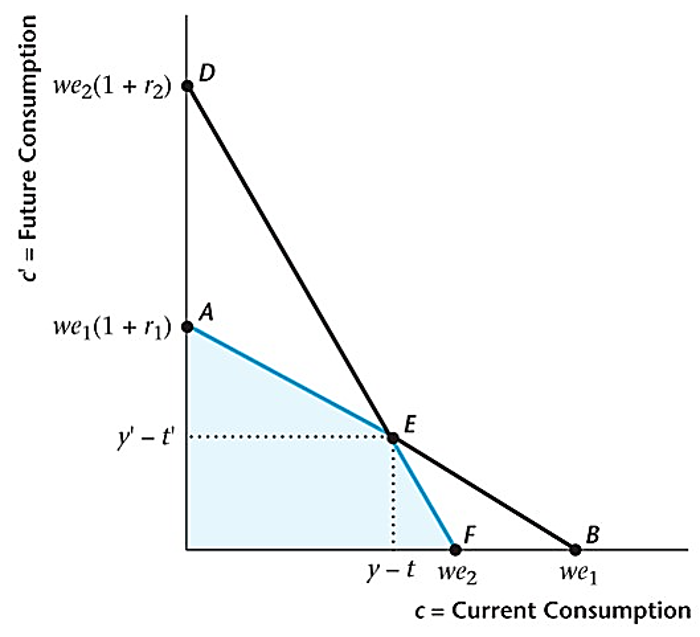
\includegraphics[scale=0.5]{Figures/W_Fig_10pt1.png}
\end{figure}
We borrow to the right of E, lend to the left.  AEF is our budget constraint. (DE and EB are irrelevant)
\end{frame}

\begin{frame}
\frametitle[alignment=center]{Kinked Budget Constraints}
$$c+s=y-t$$
\begin{itemize}
\item When you have heterogeneous indifference curves, they tend to stack at the kink (uniform preferences that would have been different all end up on that point, which ``sticks out")
\bigskip
\item Should get many people who are neither borrowers nor lenders
\end{itemize}
\end{frame}

\begin{frame}
\frametitle[alignment=center]{Effects of a Tax Cut to a Consumer with Different Borrowing and Lending Rates}
\begin{figure}
\centering
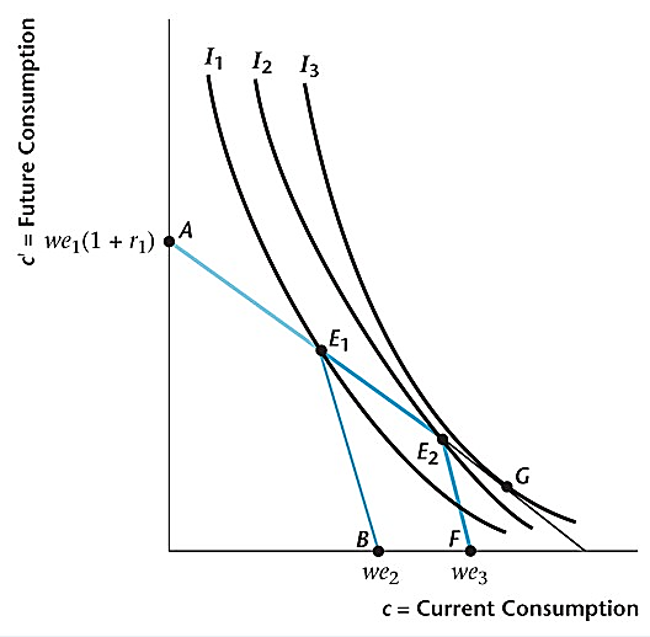
\includegraphics[scale=0.5]{Figures/W_Fig_10pt2.png}
\end{figure}
No Ricardian Equivalence!  Higher income today, lower income tomorrow but $c_1\uparrow$, $c_2\downarrow$ (consumption bundles are endowments $E_1$ and $E_2$, b/c consumer is at a corner solution/wishes he could consume even more today!)
\end{frame}

\begin{frame}
\frametitle[alignment=center]{Policy}
\begin{itemize}
\item Credit market imperfections can help break Ricardian equivalence
\bigskip
\item Perhaps a deficit-financed lump-sum tax cut can increase consumption today, decrease it tomorrow!
\bigskip
\item In doing so, govt is essentially a bank giving loans
\bigskip
\item Whether this increases efficiency/happiness depends on whether or not the kink was there for a reason (e.g. high costs of screening \& evaluating loans)
\end{itemize}
\end{frame}

\begin{frame}
\frametitle[alignment=center]{Asymmetric Information}
\begin{itemize}
\item What causes a kink?
\bigskip
\item One answer is ``asymmetric information:" one party has more information than another
\bigskip
\item We want to create a model of asymmetric information between a consumer \& a bank \& a govt that works with Ch. 9
\end{itemize}
\end{frame}


\begin{frame}
\frametitle[alignment=center]{Model Description}
\begin{itemize}
\item We have same consumers/households as in Ch. 9
\bigskip
\item But now they deposit money (are lenders) to bank in the first period, get interest rate $r_1$.
\bigskip
\item Bank takes deposits and makes loans.  
\bigskip
\item Problem!  Some fraction $1-a$ borrowers are ``bad," get zero income and default on their loan
\bigskip
\item Borrowers know they are bad, but bank does not 
\bigskip
\item Two types: good and bad borrowers
\bigskip
\item Borrowers choose loan quantity $L$, bad borrowers imitate good so they also choose $L$.  
\bigskip
\item If pay back, pay back at $r_2>r_1$
\end{itemize}
\end{frame}

\begin{frame}
\frametitle[alignment=center]{Model Description-II}
\begin{itemize}
\item For each $L$ deposits, bank has $a$ good borrowers and $1-a$ bad borrowers
\bigskip
\item Pays out $L(1+r_1)$ (pays depositors for all loans, good and bad)
\bigskip
\item But only recieves $aL(1+r_2)$
\bigskip
\item Bank profits are:
\begin{align*}
\pi & =aL(1+r_2)-L(1+r_1)\\
 & = L(a(1+r_2)-(1+r_1))
\end{align*}
\item In equilibrium, $\pi=0$ (competition between banks) so:
$$r_2^*=\frac{1+r_1}{a}-1$$
\end{itemize}
\end{frame}

\begin{frame}
\frametitle[alignment=center]{Model Description-III}
$$r_2^*=\frac{1+r_1}{a}-1$$
\begin{itemize}
\item A few things to notice about the equilibrium interest rate(s)!
\begin{itemize}
\item If everyone a good borrower, $a=$, so $r_2^*=1$
\bigskip
\item If bad borrowers, $r_2^*>r_1$
\bigskip
\item Implicitly, good borrowers pay for bad
\bigskip
\item Preventing default (as in student loans!) helps people who wouldn't have defaulted
\end{itemize}
\item An increase in non-creditworthy/bad borrowers increases borrowing interest rates (sharpens the kink)
\end{itemize}
\end{frame}

\begin{frame}
\frametitle[alignment=center]{Increase in Bad Borrowers Sharpens the Kink!}
\begin{figure}
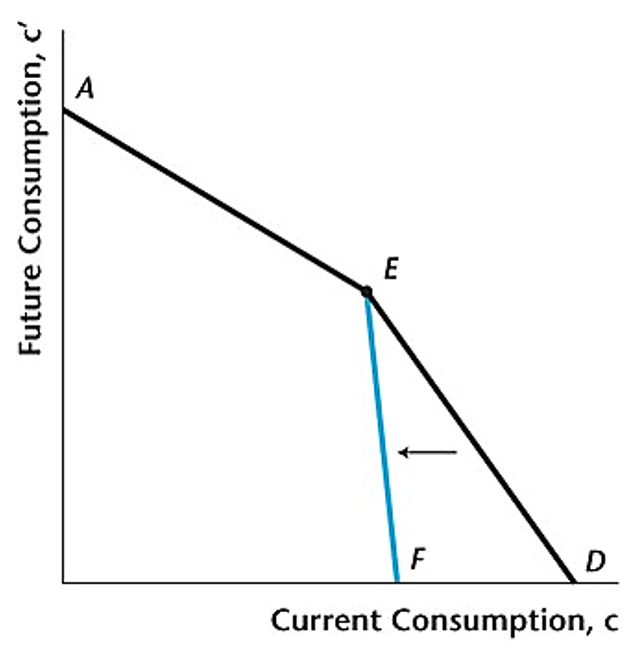
\includegraphics[scale=0.5]{Figures/W_Fig_10pt3.png}
\end{figure}
Bad news for anyone to the right of $E$!
\end{frame}

\begin{frame}
\frametitle[alignment=center]{Credit Spreads Fluctuate Wildly!}
\begin{figure}
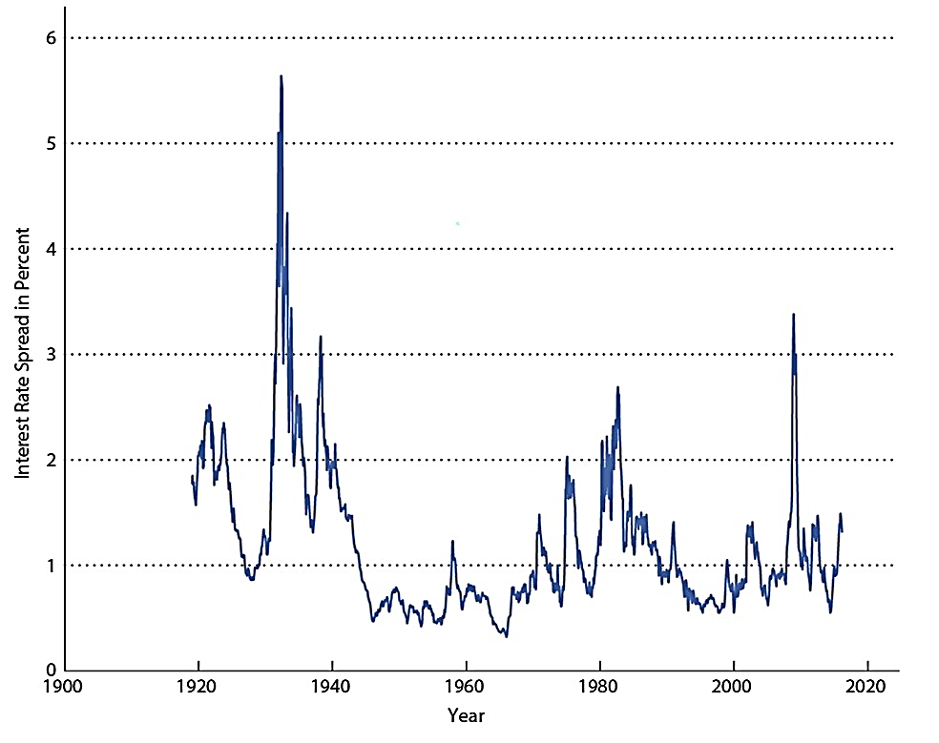
\includegraphics[scale=0.5]{Figures/W_Fig_10pt4.png}
\end{figure}
BAA-rated bonds minus AAA rated bonds (unconditional pr(default in next year)$\approx$0.02\% and 0.37\% respectively) 
 \end{frame}

\begin{frame}
\frametitle[alignment=center]{Another possibility-limited commitment}
\begin{itemize}
\item In the previous model, we emphasized \emph{asymmetric information}
\bigskip
\item In this model, we will use a model of \emph{limited commitment}
\bigskip
\item The idea behind limited commitment is that we can't promise to do what is in our interest not to do!
\bigskip
\item Imagine everyone can default freely--can a loan market still exist?
\bigskip
\item Yes!  A good example is home loans--\emph{collateral} helps make it in your interest to keep your promise
\bigskip
\item Much of the short-term money market in the U.S. depends on ``repo" loans, which use treasuries as collateral 
\end{itemize}
 \end{frame}

\begin{frame}
\frametitle[alignment=center]{Limited Commitment Model-I}
\begin{itemize}
\item Idea:  now consumers own some asset, such as housing $H$, which has a value $pH$ in the future
\bigskip
\item But can't sell $H$ quickly!  (``illiquid" asset)
\bigskip
\item Their lifetime wealth is:
$$we=y-t+\frac{y'-t'+pH}{1+r}$$
\item However, they have a \textbf{borrowing constraint}: they can't borrow more than the collateral they post $pH$:
$$-s(1+r)\leq pH$$
\item So their maximum borrowing is less than or equal to what they can pay back if the collateral is reposessed
\bigskip
\item This gives the constraint on consumption:
$$c\leq y-t+\frac{pH}{1+r}$$
\item Let's graph it!
\end{itemize}
 \end{frame}

\begin{frame}
\frametitle[alignment=center]{Limited Commitment with Collateral}
\begin{figure}
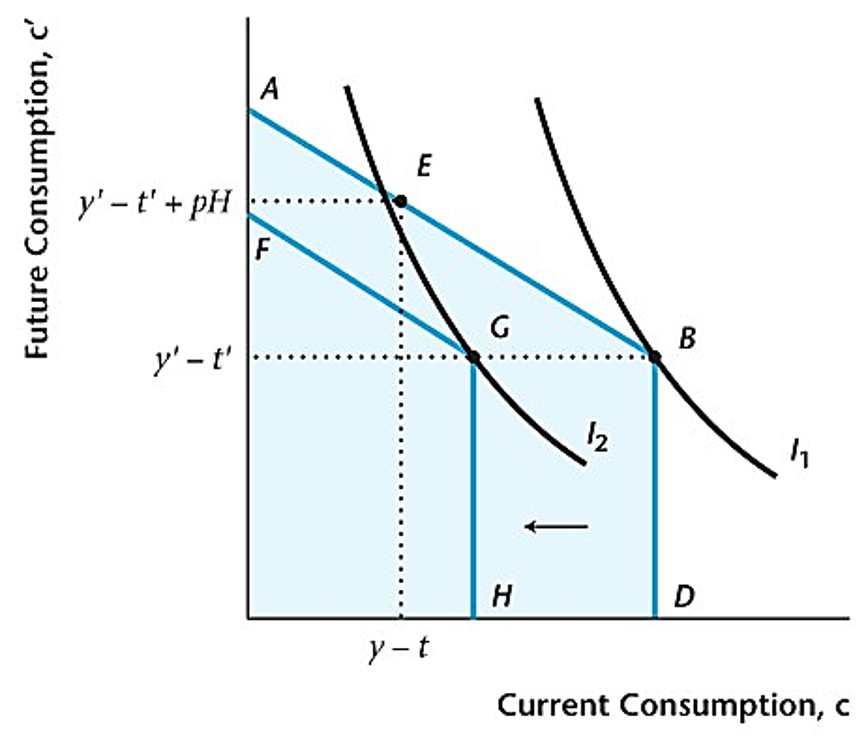
\includegraphics[scale=0.5]{Figures/W_Fig_10pt5.png}
\end{figure}
Now kink is inifinite!  A shift in value of collateral $p$ shifts in borrower's budget constraint like a decrease in $a$ did before! 
 \end{frame}

\begin{frame}
\frametitle[alignment=center]{Data Check!}
\begin{itemize}
\item Many venues of causality, but let's check the relationship between housing prices and consumption!
\end{itemize}
 \end{frame}


\begin{frame}
\frametitle[alignment=center]{Housing Market and Consumption}
\begin{figure}
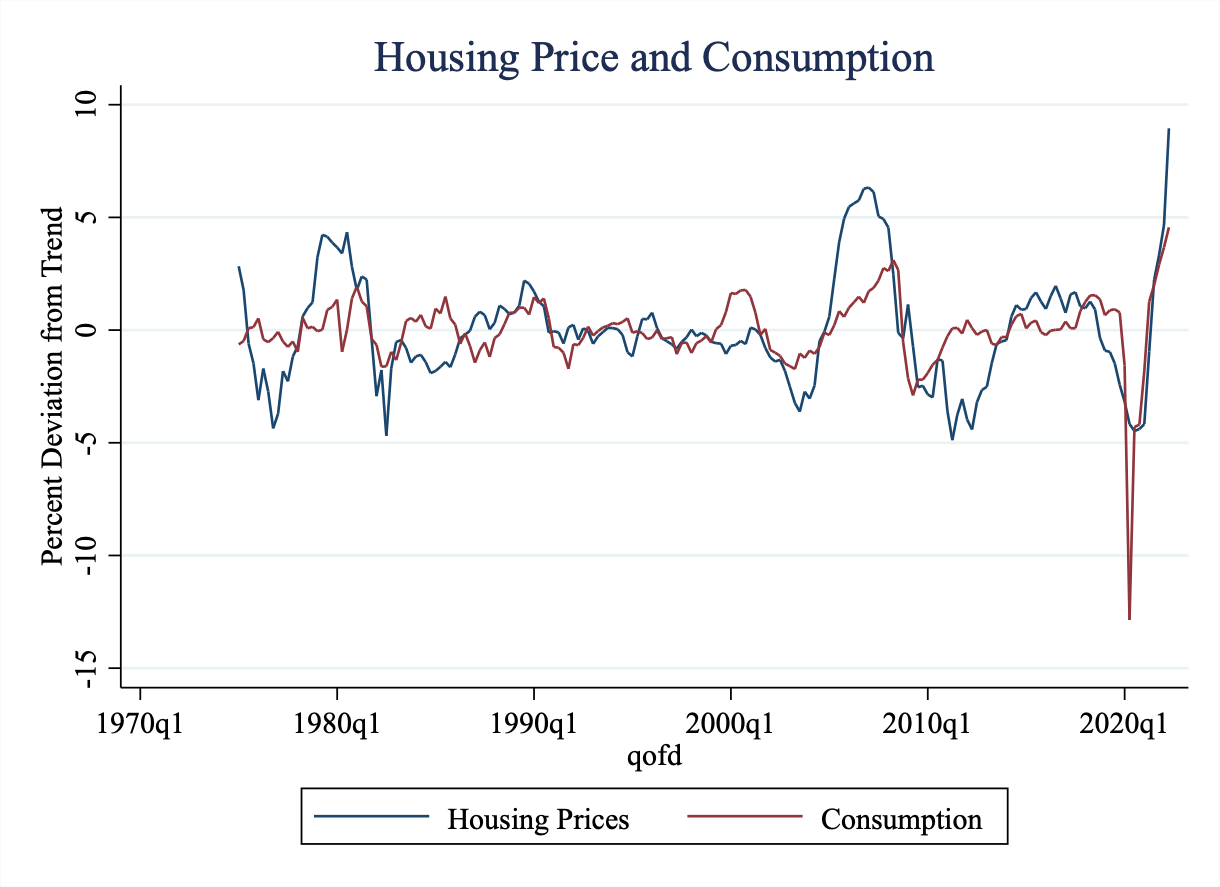
\includegraphics[scale=0.25]{Figures/H1.png}
\end{figure}
Housing in the U.S.
 \end{frame}


\begin{frame}
\frametitle[alignment=center]{Housing Market and Consumption}
\begin{figure}
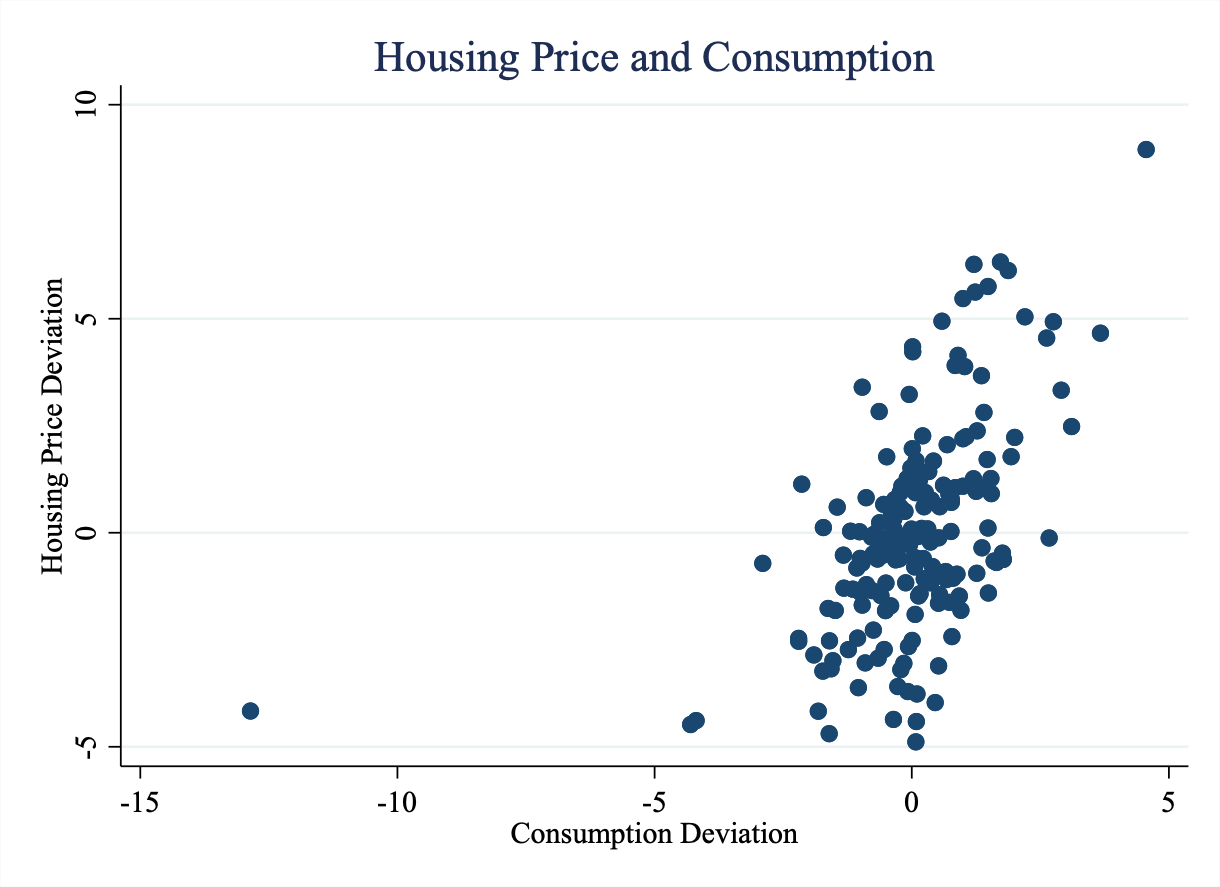
\includegraphics[scale=0.25]{Figures/H2.png}
\end{figure}
(Covid is big outlier!)
 \end{frame}



\begin{frame}
\frametitle[alignment=center]{Social Security}
\begin{itemize}
\item Many ways to run a retirement system
\bigskip
\item U.S. uses a ``pay-as-you-go" system, in which young pay for old (no ``lock box")
\bigskip
\item Could alternatively have a ``fully funded" system
\bigskip
\item Let's look at/model the consequences of each!
\bigskip
\item Caveat:  I think a lot of the economic focus on social security by economic theory is a little silly, showing something is mathematically possible, even if irrelevant
\bigskip
\item However, the setup is valuable
\end{itemize}
 \end{frame}

\begin{frame}
\frametitle[alignment=center]{Thinking about SS}
\begin{itemize}
\item Population grows at rate $n$:
$$N'=(1+n)N$$
\item Consumers receive $y$ when young and $y'$ when old
\bigskip
\item Up to period $T$, there is no social security system, taxes are zero
\bigskip
\item After period $T$, social security comes in and gives the old $b$ units of consumption
\bigskip
\item Tax for young is $t=b/(1+n)$, tax for old is $t'=-b$
\bigskip
\item Claim: this is ``free money" bc BC of old increases by $b$, but young by $b/(1+n)$
\bigskip
\item Taking advantage of ``Ponzi scheme" of population growth
\end{itemize}
 \end{frame}


\begin{frame}
\frametitle[alignment=center]{BC Old}
\begin{figure}
\centering
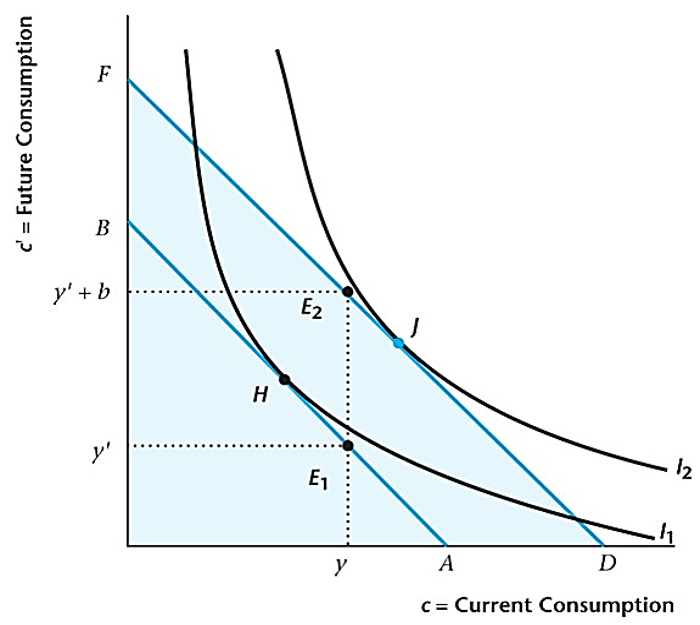
\includegraphics[scale=0.5]{Figures/W_Fig_10pt8.png}
\end{figure}
The old get a straight benefit of $b$
 \end{frame}


\begin{frame}
\frametitle[alignment=center]{BC Young}
\begin{figure}
\centering
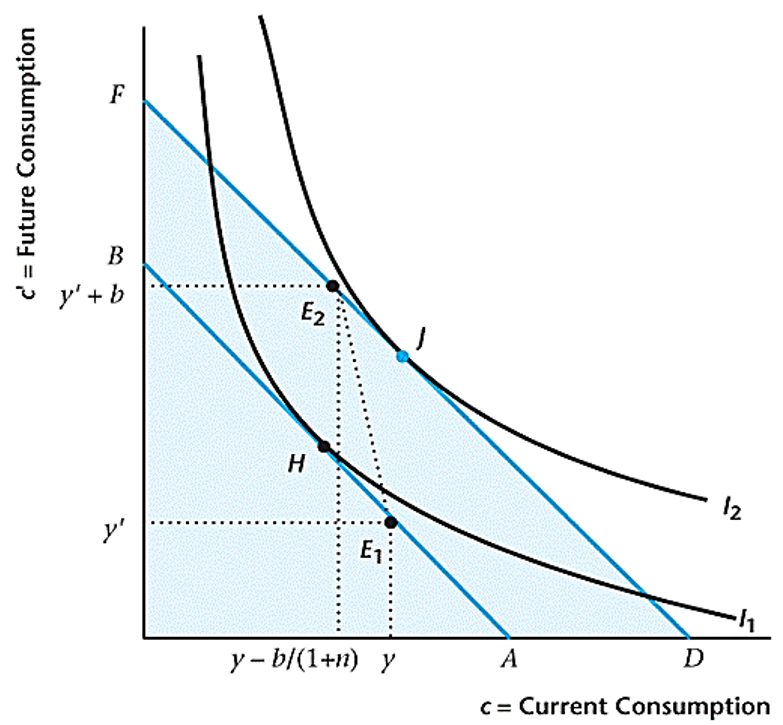
\includegraphics[scale=0.5]{Figures/W_Fig_10pt9.png}
\end{figure}
The young lose $b/(1+n)$, but gain $b$
 \end{frame}
 
 \begin{frame}
\frametitle[alignment=center]{Consumer Wealth Change}
\begin{itemize}
\item Consumer's lifetime wealth:
\begin{align*}
we & =y-\frac{b}{1+n}+\frac{y'+b}{1+r}\\
 & = y+\frac{y'}{1+r}+\frac{b(n-r)}{(1+r)(1+n)}
\end{align*}
\item If $n>r$, then everyone better off
\bigskip
\item If $n<r$, then old better off, young worse off
\bigskip
\item $r>n$ in data, by far.
\bigskip
\item But core idea of Social Security is that govt can let old trade with young
\end{itemize}
 \end{frame}

 \begin{frame}
\frametitle[alignment=center]{Fully Funded Social Security}
\begin{itemize}
\item Now let's turn to fully-funded Social Security (forced savings)
\bigskip
\item In our typical model, it only makes people worse off
\bigskip
\item If it binds, then consumer would be happier to consume more when young
\bigskip
\item If it didn't bind, then it did nothing!
\bigskip
\item But Social Security may be a \emph{commitment device} for the government for low-savers who it would otherwise bail out of destitution
\end{itemize}
 \end{frame}

\begin{frame}
\frametitle[alignment=center]{Fully-Funded Social Security}
\begin{figure}
\centering
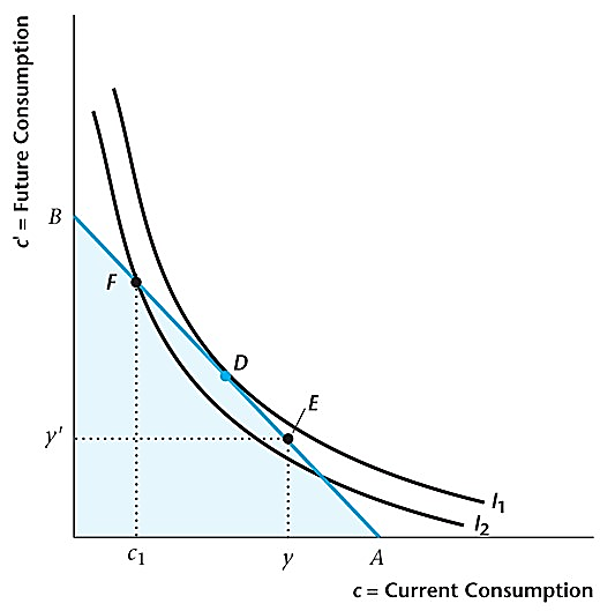
\includegraphics[scale=0.7]{Figures/W_Fig_10pt10.png}
\end{figure}
Forced savings does nothing in our baseline model, just turns savers into borrowers
 \end{frame}

 \begin{frame}
\frametitle[alignment=center]{Conclusions}
\begin{itemize}
\item We now have a model of imperfect credit markets
\bigskip
\item Asymmetric information and limited commitment help ``kink" the budget constraint: higher rates for borrowing than lending
\bigskip
\item That tends to make people consume the endowment
\bigskip
\item Reason to think it might be important (data on credit spreads, housing and consumption)
\bigskip
\item Thinking about social security
\begin{itemize}
\item Pay as you go could make everyone better off (under unrealistic assumptions)
\item Fully-funded doesn't make sense (forced savings) unless external motivation like govt commitment mechanism
\end{itemize}
\end{itemize}
 \end{frame}


\end{document}